Durch das kombinieren aller Photonenkandidaten, wie es in Abschnitt \ref{s2s2s1} gezeigt wurde, ist ein gro{\ss}er Anteil der rekonstruierten Massen aus nicht korreliert Paaren.
Das hei{\ss}t, dass die beiden Photonenkandidaten nicht zusammenh{"a}ngen {\"u}ber beispielsweise einen Zerfall.
Um diesen unkorrelierten Untergrund abzusch{\"a}tzen werden im sogenannten Eventmixing Photonenkandidaten aus unterschiedlichen Events zusammen kombiniert, da so sicher keine Verbindung zwischen den beiden Photonenkandidaten besteht.
Abbildung \ref{figUncorrBkg} zeigt das Ergebnis des Eventmixings f{\"u}r einen gew{\"a}hlten $p_{\rm{T}}$-Bereich.
\begin{figure}[thp]
\centering
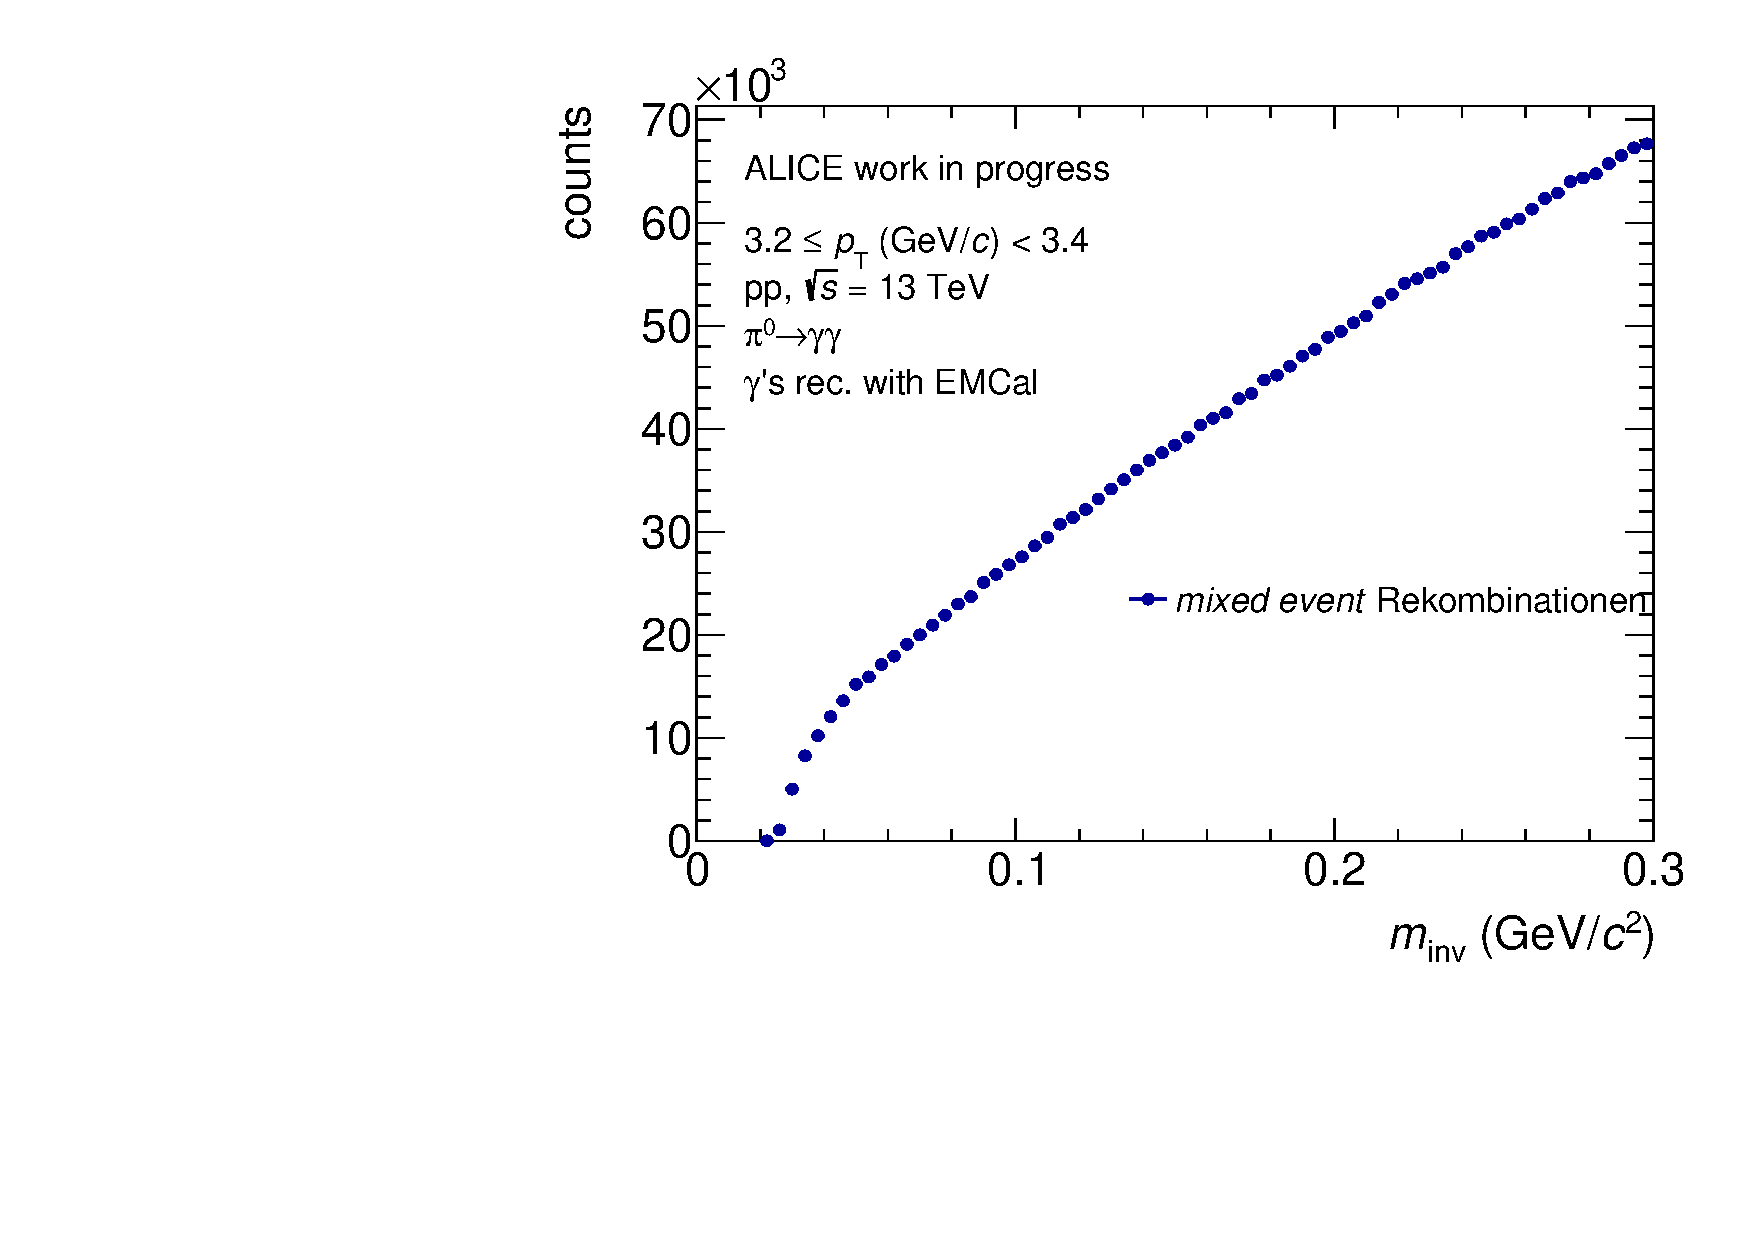
\includegraphics[width=.6\linewidth]{hUncorrBkg.pdf}
\caption{Kombinationen von Photonenkandidaten aus unterschiedlichen Kollisionen, die keine Korrelationen zueinander haben, weshalb auch kein Peak im Bereich der $\pi^{0}$-Masse zu sehen ist. Dies dient als Grundlage zur Bestimmung des unkorrelierten Untergrunds.}
\label{figUncorrBkg}
\end{figure}
\newline
Abbildung \ref{figUncorrBkg} zeigt die invariante Massenverteilung f\"ur \textit{mixed events} in einem ausgew{\"a}hlten $p_{\rm{T}}$-Bereich..
Diese Verteilung weist keinen Peak auf und hat eine gr{\"o}{\ss}ere Anzahl Eintr{\"a}ge, als die Verteilung aus dem selben Events.
Aufgrund der gr{\"o}{\ss}ere Anzahl Eintr{\"a}ge muss die \textit{mixed event} Verteilung an die der \textit{same events} skaliert werden.
Die Skalierung erfolgt im rechten Bereich au{\ss}erhalb des $\pi^{0}$-Peaks und es ergibt sich f{\"u}r den Skalierungsfaktor:
\begin{align}
\label{eqBackSkalierung}
\alpha &= \frac{\sum_{i \neq j}\sum_{n}m_{\text{inv}}\left( \gamma^{(n)}_{i},\gamma^{(n)}_{j}\right) }{\sum_{i,j}\sum_{n \neq m}m_{\text{inv}}\left( \gamma^{(n)}_{i},\gamma^{(m)}_{j}\right) }
\end{align}
Die oberen Indizes stehen hierbei f{\"u}r das Event, aus dem ein Photon kommt.\newline
\begin{figure}[thp]
\centering
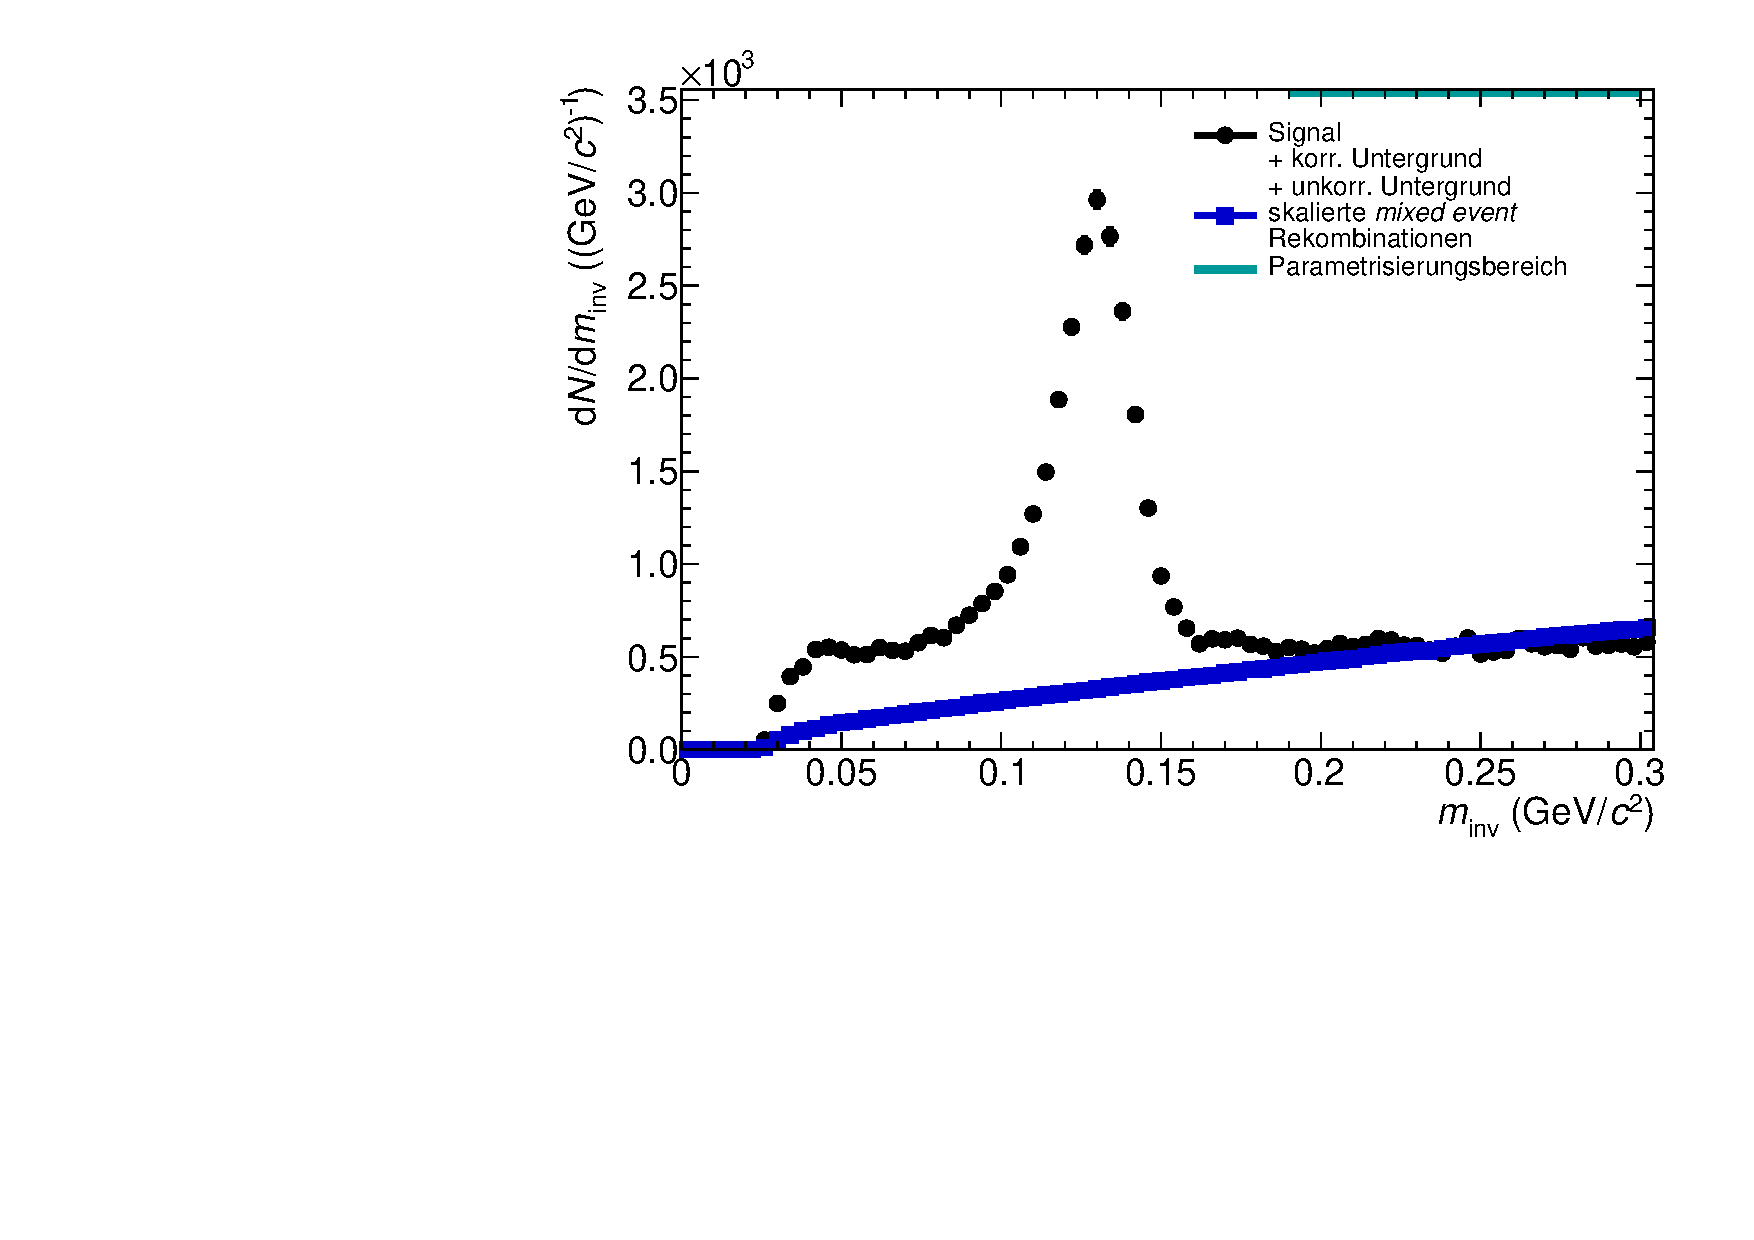
\includegraphics[width=.6\linewidth]{hUncorrBkgNorm.pdf}
\caption{Nach Gleichung \ref{eqBackSkalierung} skalierte {\it mixed event} Rekombinationen aus Abbildung \ref{figUncorrBkg} als Absch{\"a}tzung des unkorrelierten Untergrunds zusammen aufgetragen mit Signal zuz{\"u}glich beiden Untergrundkomponenten wie in Abbildung \ref{figSignalPlusBkg}.}
\label{figUncorrBkgNorm}
\end{figure}
\newline
Das Resultat der Skalierung ist in Abbildung \ref{figUncorrBkgNorm} zu sehen, wo zus{\"a}tzlich noch das Signal inklusiver beider Untergr{\"u}nde eingezeichnet ist, um besser erkennen zu k{\"o}nnen, wie sich der abgesch{\"a}tzte korrelierte Untergrund relativ zum gesamten Signal verh{\"a}lt.
Das es sich hierbei nur um eine Absch{\"a}tzung handelt kann daran ausgemacht werden, dass um $m_{\text{inv}} = 0,3 (\text{GeV/}c)$ der unkorrelierte Untergrund gr{\"o}{\ss}er ist, als das Signal mit beiden Untergrundkomponenten, was bedeutet, dass nach Abzug des unkorrelierten Untergrunds das Signal mit korreliertem Untergrund dort negativ w{\"a}re, was physikalisch nicht sinnvoll ist.
\begin{figure}[tbp]
\centering
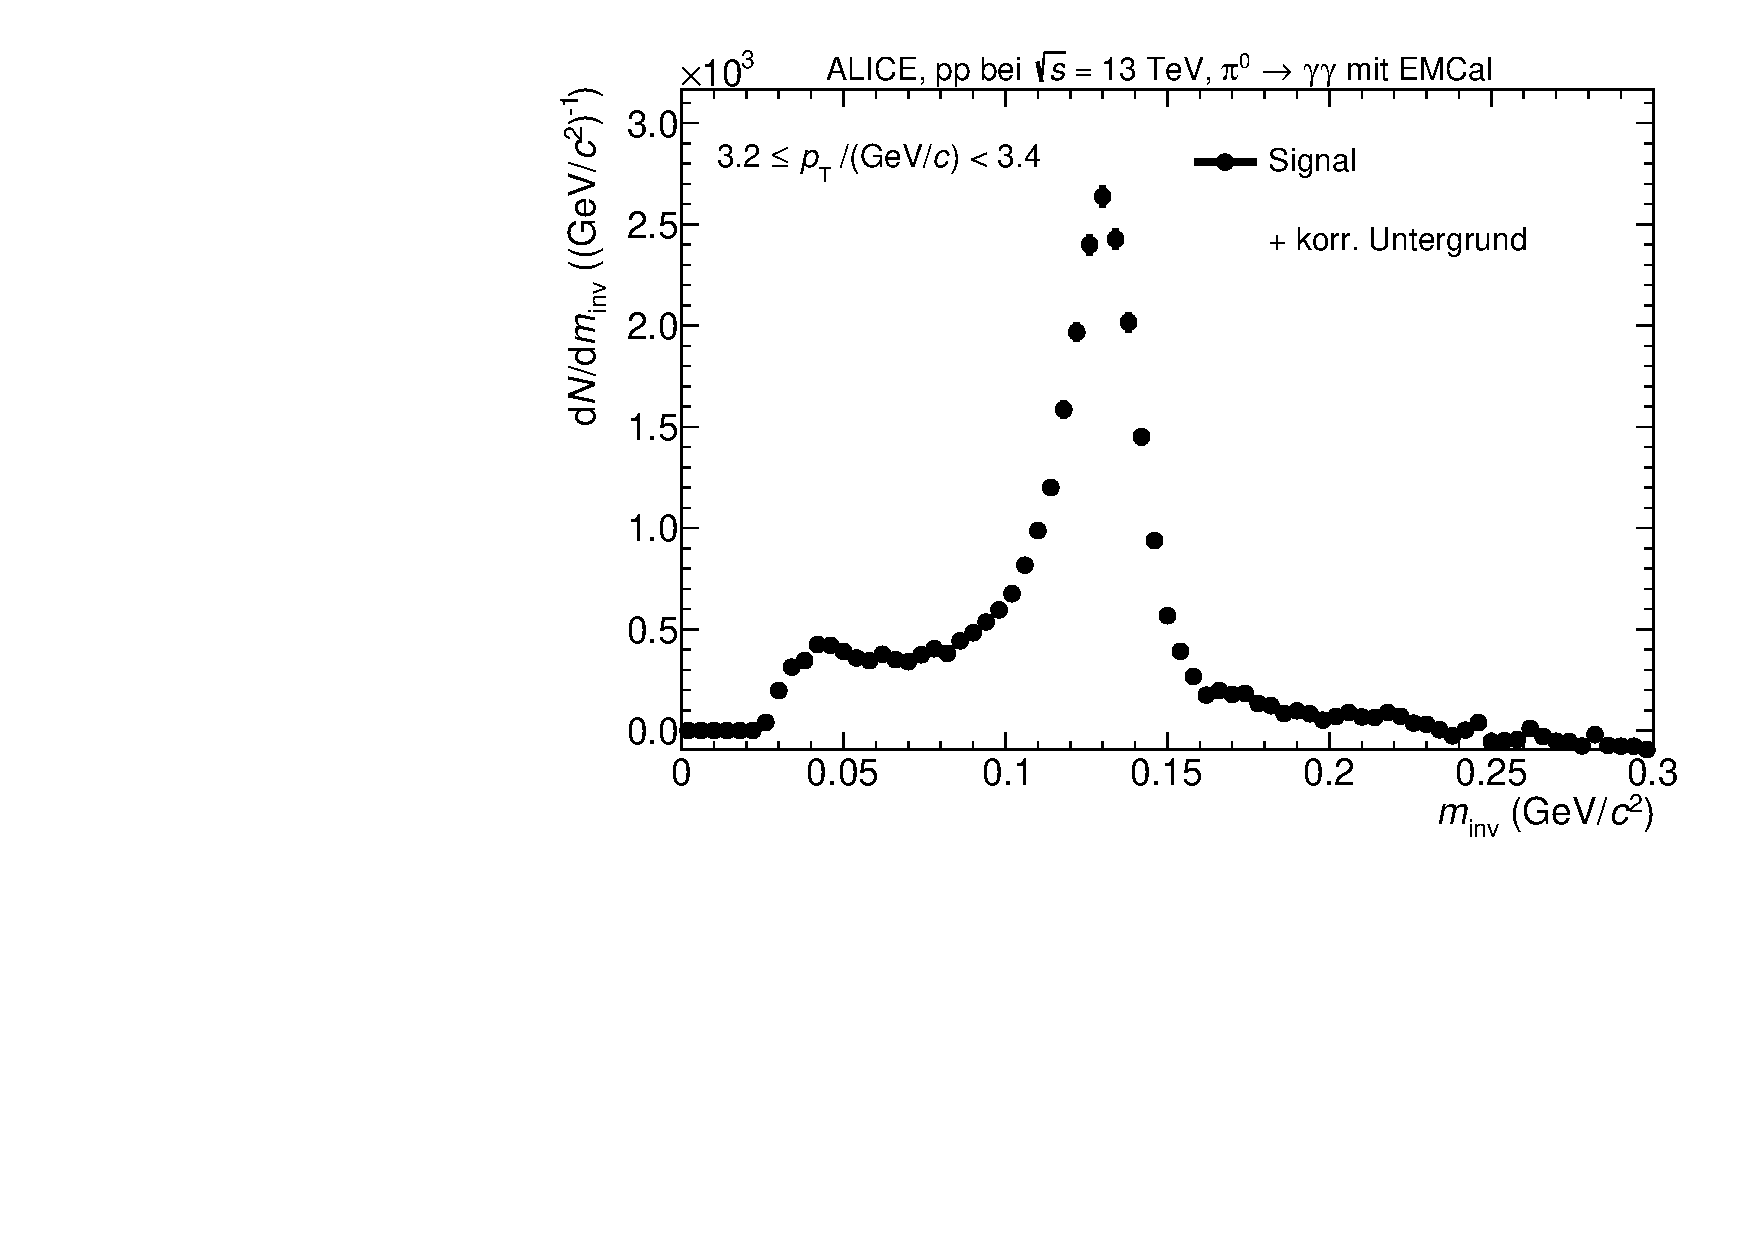
\includegraphics[width=.6\linewidth]{hInvMass_Data.pdf}
\caption{Signal nach Abzug des unkorrelierten Untergrunds.}
\label{figInvMass_Data}
\end{figure}
\newline
Abbildung \ref{figInvMass_Data} zeigt das Signal mit korreliertem Untergrund, nachdem also der unkorrelierte Untergrund abgezogen wurde.
Die Absch\"atzung des korrelierten Untergrunds wird in den folgenden Abschnitten f\"r die beiden zuvor erw\"ahnte Methoden durchgef\"uhrt.